%%%%%%%%%%%%%%%%%%%%%%%%%%%%%%%%%%%%%%%%%
% Beamer Presentation
% LaTeX Template
% Version 1.0 (10/11/12)
%
% This template has been downloaded from:
% http://www.LaTeXTemplates.com
%
% License:
% CC BY-NC-SA 3.0 (http://creativecommons.org/licenses/by-nc-sa/3.0/)
%
%%%%%%%%%%%%%%%%%%%%%%%%%%%%%%%%%%%%%%%%%

%----------------------------------------------------------------------------------------
%	PACKAGES AND THEMES
%----------------------------------------------------------------------------------------

\documentclass{beamer}

\mode<presentation> {

\usetheme{Szeged}

\usecolortheme{seahorse}

\setbeamertemplate{navigation symbols}{}

}

\usepackage[spanish]{babel}
\usepackage[utf8]{inputenc}
\usepackage{graphicx}
\usepackage{booktabs}
\usepackage[spanish]{babel}

%----------------------------------------------------------------------------------------
%	TITLE PAGE
%----------------------------------------------------------------------------------------

\title[Métodos y Técnicas de Gamificación en Educación]{Métodos y Técnicas de Gamificación Implementadas en Educación: Revisión Sistemática\\ Presentación de Avances} % The short title appears at the bottom of every slide, the full title is only on the title page

\author{Luis Angel Hernández Lázaro} % Your name
\institute[C.I.M.A.T. A.C.] % Your institution as it will appear on the bottom of every slide, may be shorthand to save space
{
Centro de Investigación en Matemáticas A.C. Unidad Zacatecas \\ % Your institution for the title page
\medskip
\textit{luis.hernandez@cimat.com} % Your email address
}
\date{\today} % Date, can be changed to a custom date

\begin{document}

%----------------------------------------------------------------------------------------
%	PRESENTATION
%----------------------------------------------------------------------------------------
\begin{frame}
\titlepage
\end{frame}

\begin{frame}
\frametitle{Agenda}
\tableofcontents 
\end{frame}

%----------------------------------------------------------------------------------------
%	PRESENTATION SLIDES
%----------------------------------------------------------------------------------------

%------------------------------------------------
\section{Introducción} %
%------------------------------------------------

\begin{frame}
	\frametitle{Motivación}
	Elegí este tema debido al interés e el área para aplicar técniacs o métodos de gamificación en la educación, con el objetivo de motivar el aprendizaje de los estudiantes y mejorar su desempeño académico.
	\\~\\
	
	\begin{figure}
		\begin{center}
			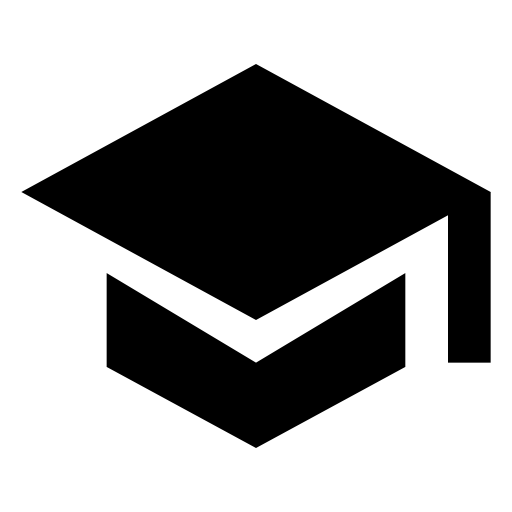
\includegraphics[scale=0.1]{images/2icons/student.png}
			\label{student}
		\end{center}
	\end{figure}
\end{frame}

\begin{frame}
	\frametitle{BackGround}
	.\\~\\
\end{frame}

%------------------------------------------------
\section{Revisión Sistemática} %
%------------------------------------------------
\begin{frame}
	\frametitle{El Proceso de la Revisión Sistemática}
	
	\begin{figure}[H]
		\begin{center}
			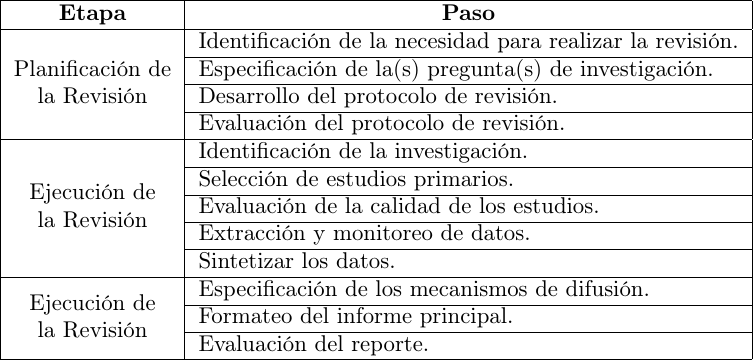
\includegraphics[scale=0.4]{images/1document/steps.png}
			\caption{Etapas y Pasos en una Revisión Sistemática}
			\label{Pasos}
		\end{center}
	\end{figure}
	
\end{frame}
%------------------------------------------------
\subsection{Planeación de la Revisión} %
%------------------------------------------------

%------------------------------------------------
\subsubsection{Protocolo} %
%------------------------------------------------

%------------------------------------------------
\subsubsection{Indenficación de la Necesidad de la Revisión Sistemática} %
%------------------------------------------------

%------------------------------------------------
\subsubsection{Especificación de las Preguntas de Investigación} %
%------------------------------------------------

%------------------------------------------------
\subsection{Ejecución de la Revisión} %
%------------------------------------------------

%------------------------------------------------
\subsubsection{Selección de las Fuentes de Investigación} %
%------------------------------------------------

%------------------------------------------------
\subsubsection{Procedimiento de Selección de Estudios} %
%------------------------------------------------

%------------------------------------------------
\subsubsection{Evaluación de la Calidad de Estudios} %
%------------------------------------------------

%------------------------------------------------
\subsubsection{Extracción y Monitoreo de la Información} %
%------------------------------------------------

%------------------------------------------------
\subsubsection{Sístensis de la Información} %
%------------------------------------------------

%------------------------------------------------
\subsection{Reporte de Resultados} %
%------------------------------------------------

%------------------------------------------------
\subsubsection{Revisiones Literarias} %
%------------------------------------------------

%------------------------------------------------
\subsubsection{Métodos y Técnicas Aplicados} %
%------------------------------------------------

%------------------------------------------------
\subsubsection{Evaluación del Reporte} %
%------------------------------------------------

%------------------------------------------------
\section{Conclusiónes} %
%------------------------------------------------

\begin{frame}
\frametitle{Objetivos: General y Específicos}
Como parte de la definición de nuestro Objetivo General del estudio tenemos:\\~\\
\begin{description}
	\item[Definir] el estado del arte actual del uso de técnicas de Gamificación en la educación tradicional (Aula, Alumno, Profesor), para descubrir las diferentes técnicas de Gamificación para implementarlas en la educación.
\end{description}

\end{frame}

%------------------------------------------------

\begin{frame}
\frametitle{Bullet Points}
\begin{itemize}
\item Lorem ipsum dolor sit amet, consectetur adipiscing elit
\item Aliquam blandit faucibus nisi, sit amet dapibus enim tempus eu
\item Nulla commodo, erat quis gravida posuere, elit lacus lobortis est, quis porttitor odio mauris at libero
\item Nam cursus est eget velit posuere pellentesque
\item Vestibulum faucibus velit a augue condimentum quis convallis nulla gravida
\end{itemize}
\end{frame}

%------------------------------------------------

\begin{frame}
\frametitle{Blocks of Highlighted Text}
\begin{block}{Block 1}
Lorem ipsum dolor sit amet, consectetur adipiscing elit. Integer lectus nisl, ultricies in feugiat rutrum, porttitor sit amet augue. Aliquam ut tortor mauris. Sed volutpat ante purus, quis accumsan dolor.
\end{block}

\begin{block}{Block 2}
Pellentesque sed tellus purus. Class aptent taciti sociosqu ad litora torquent per conubia nostra, per inceptos himenaeos. Vestibulum quis magna at risus dictum tempor eu vitae velit.
\end{block}

\begin{block}{Block 3}
Suspendisse tincidunt sagittis gravida. Curabitur condimentum, enim sed venenatis rutrum, ipsum neque consectetur orci, sed blandit justo nisi ac lacus.
\end{block}
\end{frame}

%------------------------------------------------

\begin{frame}
\frametitle{Multiple Columns}
\begin{columns}[c] % The "c" option specifies centered vertical alignment while the "t" option is used for top vertical alignment

\column{.45\textwidth} % Left column and width
\textbf{Heading}
\begin{enumerate}
\item Statement
\item Explanation
\item Example
\end{enumerate}

\column{.5\textwidth} % Right column and width
Lorem ipsum dolor sit amet, consectetur adipiscing elit. Integer lectus nisl, ultricies in feugiat rutrum, porttitor sit amet augue. Aliquam ut tortor mauris. Sed volutpat ante purus, quis accumsan dolor.

\end{columns}
\end{frame}

\begin{frame}
\frametitle{Table}
\begin{table}
\begin{tabular}{l l l}
\toprule
\textbf{Treatments} & \textbf{Response 1} & \textbf{Response 2}\\
\midrule
Treatment 1 & 0.0003262 & 0.562 \\
Treatment 2 & 0.0015681 & 0.910 \\
Treatment 3 & 0.0009271 & 0.296 \\
\bottomrule
\end{tabular}
\caption{Table caption}
\end{table}
\end{frame}

%------------------------------------------------

\begin{frame}
\frametitle{Theorem}
\begin{theorem}[Mass--energy equivalence]
$E = mc^2$
\end{theorem}
\end{frame}

%------------------------------------------------

\begin{frame}[fragile] % Need to use the fragile option when verbatim is used in the slide
\frametitle{Verbatim}
\begin{example}[Theorem Slide Code]
\begin{verbatim}
\begin{frame}
\frametitle{Theorem}
\begin{theorem}[Mass--energy equivalence]
$E = mc^2$
\end{theorem}
\end{frame}\end{verbatim}
\end{example}
\end{frame}

%------------------------------------------------

\begin{frame}
\frametitle{Figure}
Uncomment the code on this slide to include your own image from the same directory as the template .TeX file.
%\begin{figure}
%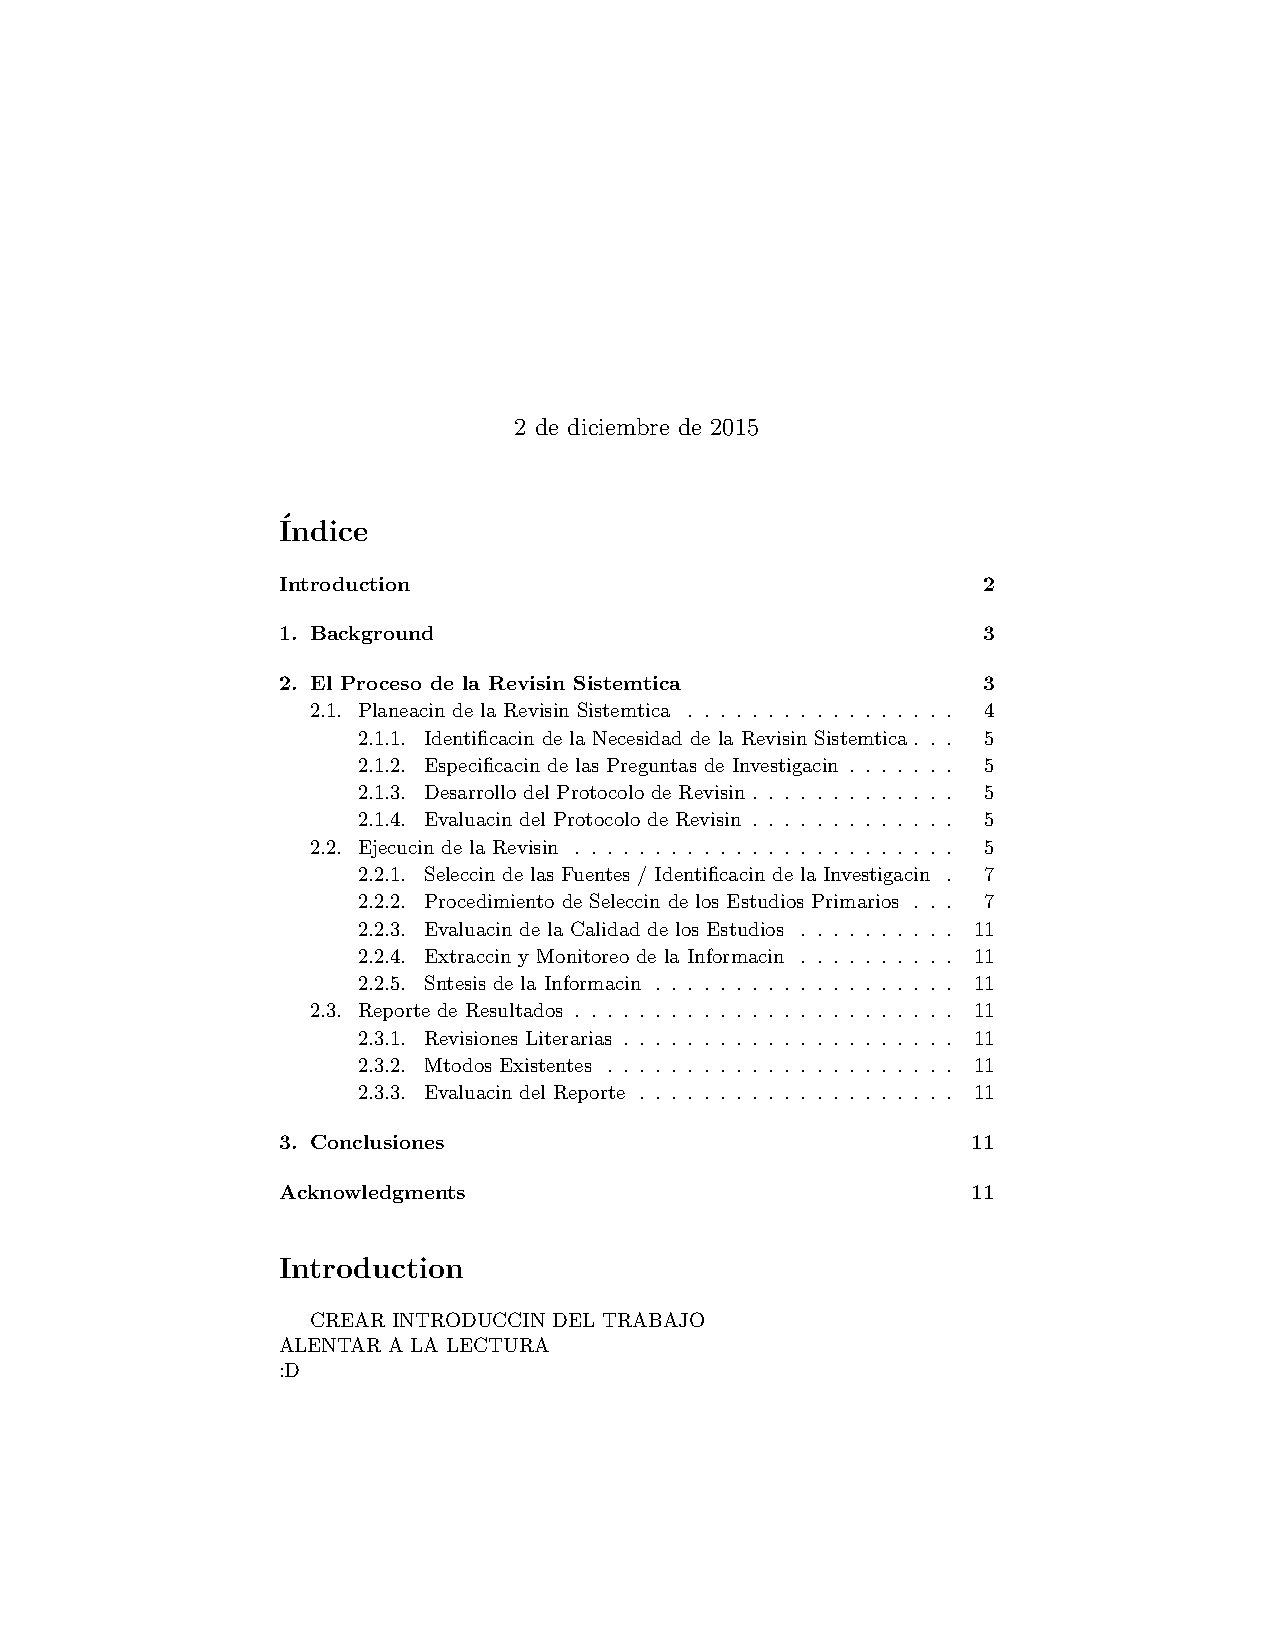
\includegraphics[width=0.8\linewidth]{test}
%\end{figure}
\end{frame}

%------------------------------------------------

\begin{frame}[fragile] % Need to use the fragile option when verbatim is used in the slide
\frametitle{Citation}
An example of the \verb|\cite| command to cite within the presentation:\\~

This statement requires citation \cite{p1}.
\end{frame}

%------------------------------------------------

\begin{frame}
\frametitle{References}
\footnotesize{
\begin{thebibliography}{99} % Beamer does not support BibTeX so references must be inserted manually as below
\bibitem[Smith, 2012]{p1} John Smith (2012)
\newblock Title of the publication
\newblock \emph{Journal Name} 12(3), 45 -- 678.
\end{thebibliography}
}
\end{frame}

%------------------------------------------------

\begin{frame}
\Huge{\centerline{The End}}
\end{frame}

%----------------------------------------------------------------------------------------

\end{document} 